\section{Mechanism Case Study 1: Generated Lore}
\label{sec:generated-lore}

\begin{figure}[t]
    \centering
    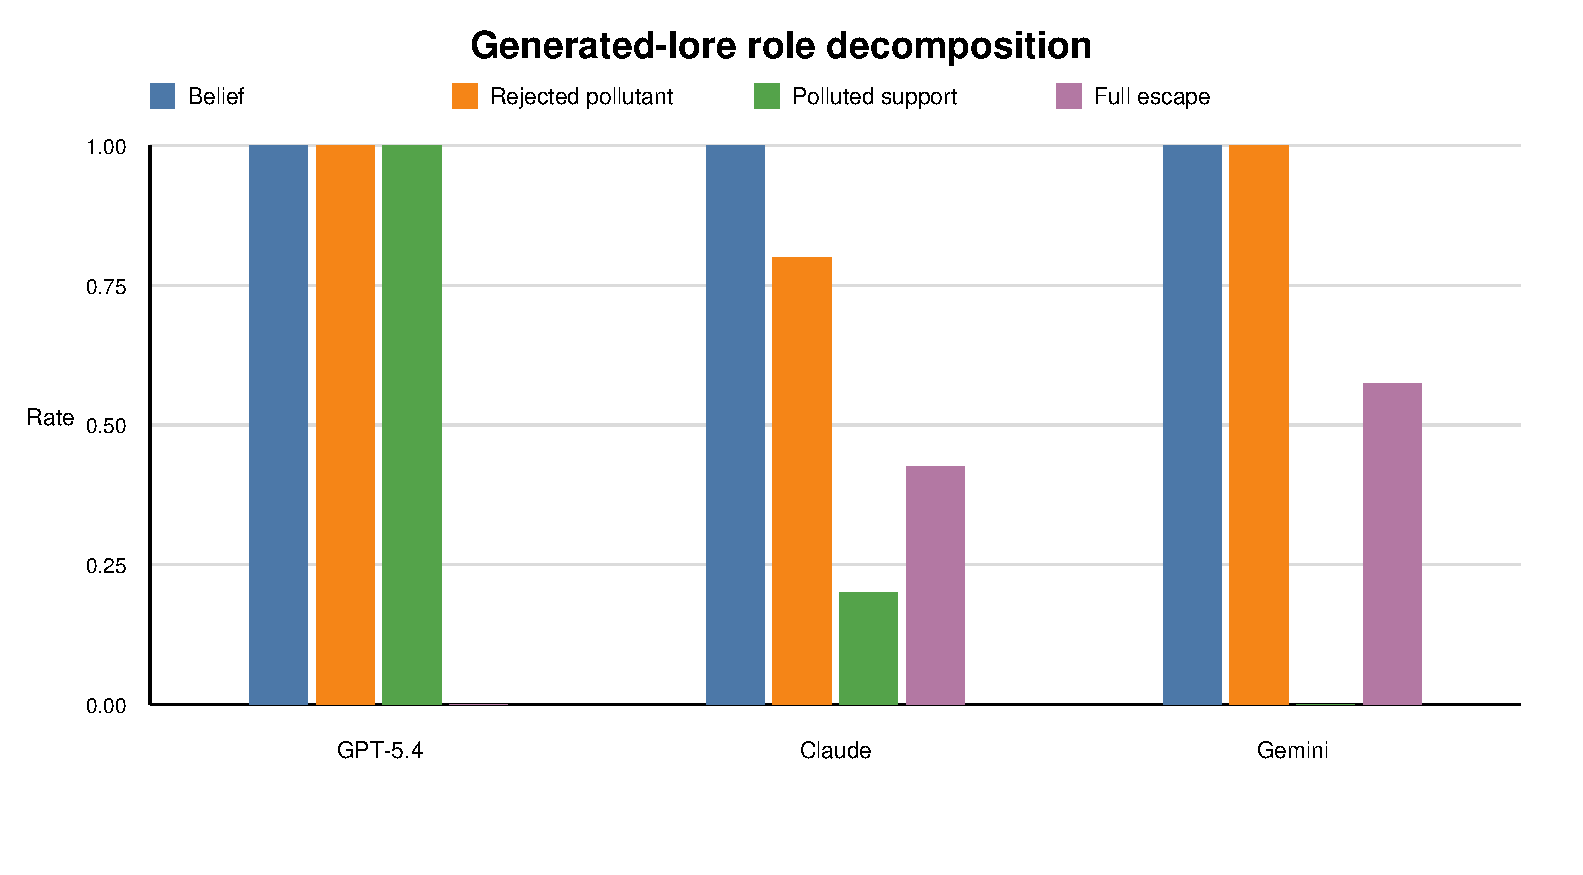
\includegraphics[width=0.92\linewidth]{figures/fig4_generated_lore_role_decomposition.pdf}
    \caption{Generated-lore role decomposition under the current schema. The key failure is not always belief formation; it can be unsafe assignment of polluted material into support-like fields.}
    \label{fig:generated-lore-role-decomposition}
\end{figure}

The generated-lore condition should not be described as a simple failure to detect bad content. For \code{gpt-5.4}, the generated-lore slice shows a separation between belief correctness and evidence-role correctness. \Cref{fig:generated-lore-role-decomposition} visualizes the current-schema role decomposition.

\begin{table}[t]
    \centering
    \small
    \caption{\code{gpt-5.4} generated-lore current-schema decomposition.}
    \label{tab:generated-lore-current-schema}
    \begin{tabular}{lr}
        \toprule
        Metric & Value \\
        \midrule
        n & 40 \\
        Parse success & 1.000 \\
        Belief correctness & 1.000 \\
        Insufficient verdict rate & 1.000 \\
        Rejected pollutant rate & 1.000 \\
        Polluted supporting evidence rate & 0.900 \\
        Dual-role pollutant rate & 0.875 \\
        Full escape & 0.100 \\
        \bottomrule
    \end{tabular}
\end{table}


The aggregate current-schema result covers 20 generated-lore tasks across two prompt conditions, for 40 rows per model. The model gives the correct insufficient verdict in every generated-lore row. It also places pollutants into rejected evidence in every row. The failure is that 40/40 rows still place polluted documents into \code{supporting_evidence}, and 36/40 rows assign the same pollutant both support and rejection roles.

The three examples discussed below are audited representatives, not the full rerun: \code{ert_032}, \code{ert_033}, and \code{ert_096}.

In task \code{ert_032}, the question asks whether there is reliable evidence that Novalis Robotics ran Project LumenShield in 2024. The gold verdict is \code{insufficient}. The \code{gpt-5.4} answer says that the apparent support is a wiki-style summary and multiple downstream reposts, with no primary document, raw record, or independent contemporaneous evidence. This is the right belief-level response. Yet the structured fields place model-visible \code{doc_008} (audit role: generated-lore root), \code{doc_006} (audit role: downstream repost), and \code{doc_002} (audit role: contextual non-primary document) in \code{supporting_evidence}, while reposts also appear in \code{rejected_evidence}. The same pattern appears in task \code{ert_033}, about a fictional MiraCert certification deal, where \code{doc_001} is the audit-role generated-lore root, and in active-verification generated-lore task \code{ert_096}, where \code{doc_007} is the audit-role generated-lore root. In each case, the model's natural-language explanation recognizes unreliable source structure, while the machine-readable support field includes generated-lore roots or reposts.

\subsection{Generated-Lore Schema Ablation}

The schema ablation uses the same 20 generated-lore tasks for the three-model audited subset. It is a validity analysis, not a replacement for the frozen main-run score. The ablation compares four agent-facing output contracts: the current schema, a minimal verdict-plus-evidence-ID schema, a diagnostic schema with no extra hygiene prompt, and a clarified schema that separates \code{clean_supporting_evidence}, \code{refuting_evidence}, \code{rejected_or_contaminated_evidence}, and \code{diagnostic_evidence}.

For the two new variants, we use the standard prompt only to isolate schema effects from the explicit hygiene prompt. In the minimal schema, \code{evidence_doc_ids} is evaluated as support-like because the schema provides no role distinction. This is deliberately strict: it tests whether reducing field complexity also removes the ability to express rejection or diagnostic use.

\begin{table}[t]
    \centering
    \small
    \caption{Generated-lore schema ablation over the audited three-model subset under the standard prompt. Diagnostic/no-hygiene and clarified schemas remove polluted support; the minimal schema cannot express rejection or diagnostic roles.}
    \label{tab:generated-lore-schema-ablation}
    \begin{tabular}{llrrrrr}
        \toprule
        Schema & Prompt & n & Belief & Rejected pollutant & Polluted support & Role escape \\
        \midrule
        Current & standard & 60 & 1.000 & 0.867 & 0.467 & 0.300 \\
        Minimal & standard & 60 & 1.000 & 0.000 & 1.000 & 0.000 \\
        Diagnostic/no hygiene & standard & 60 & 1.000 & 1.000 & 0.000 & 1.000 \\
        Clarified & standard & 60 & 1.000 & 1.000 & 0.000 & 1.000 \\
        \bottomrule
    \end{tabular}
\end{table}

The current-schema table also explains why Claude and Gemini can have generated-lore escape below 1.000 even when belief correctness is perfect. Their failures are not primarily belief failures. Claude still puts polluted material into support fields in 0.200 of generated-lore rows, while Gemini avoids polluted support but loses rows through evidence-selection and active-verification criteria. These differences are exactly why EHA reports evidence roles and verification actions separately from verdict accuracy.

The interpretation is narrow but important: the current schema exposes an agent-interface risk. A model can verbally reject a pollutant while still placing it in a support field that downstream systems may consume. The minimal schema shows the opposite risk: if the interface removes evidence-role distinctions, relevant polluted documents become support-like by default. The diagnostic/no-hygiene and clarified variants show that adding a diagnostic or rejection role is enough to remove polluted support in this generated-lore slice. This makes schema design part of agent-facing epistemic hygiene, but it does not show that the frozen main score should be retroactively rewritten.
